\documentclass[aspectratio=169]{beamer}

\usepackage{amsmath}
\usepackage{booktabs}
\usepackage{xcolor}
\usepackage[english]{babel}
%\usepackage{unicode-math}
\usepackage{mathtools}
%\usepackage{derivative}
%\usepackage{makecell}
%\usepackage{multirow}
\usepackage{siunitx}
%\usepackage{pgfplots}
\usepackage{circuitikz}
%\usepackage{appendixnumberbeamer}

\usetheme{metropolis}

%\setmainfont{Stix Two Text}
%\setmathfont{Stix Two Math}

%\pgfplotsset{compat=1.17}
\renewcommand{\familydefault}{\sfdefault}
\usetikzlibrary{arrows.meta}
\usetikzlibrary{fit}
\usetikzlibrary{positioning}
%\usetikzlibrary{shapes.geometric}
%\usetikzlibrary{shapes.misc}
%\usepgfplotslibrary{groupplots}

\DeclarePairedDelimiter{\ceil}{\lceil}{\rceil}
\DeclarePairedDelimiter{\floor}{\lfloor}{\rfloor}
\DeclarePairedDelimiter{\abs}{\lvert}{\rvert}
\DeclarePairedDelimiter{\norm}{\lVert}{\rVert}
\DeclarePairedDelimiter{\bra}{\langle}{\rvert}
\DeclarePairedDelimiter{\ket}{\lvert}{\rangle}
\DeclarePairedDelimiter{\expval}{\langle}{\rangle}
\DeclarePairedDelimiter{\norder}{\mathcolon}{\mathcolon}
\DeclarePairedDelimiter{\anorder}{\typecolon}{\typecolon}
	
\newcommand{\laplace}{\mbfnabla^2}
\newcommand{\trans}{{\scriptscriptstyle\mathsf{T}}}

\newcommand{\conv}{\ast}
\newcommand{\vdot}{\cdot}
\newcommand{\vcross}{\vectimes}
\newcommand{\vb}[1]{\symbfup{#1}}
\newcommand{\vu}[1]{\hat{\vb{#1}}}
\newcommand*\dd[2][\relax]{\mathop{\ifx\relax#1\odif{#2}\else \odif[order={#1}]{#2}\fi}}

\newcommand{\vacket}{\ket*{0}}
\newcommand{\vacbra}{\bra*{0}}

\DeclareMathOperator{\trace}{Tr}
\DeclareMathOperator{\sinc}{sinc}

\AtBeginDocument{
	\let\Re\relax
	\let\Im\relax
	\DeclareMathOperator{\Re}{Re}
	\DeclareMathOperator{\Im}{Im}

	\renewcommand{\div}{\mathop{\mbfnabla\vdot}}
	\newcommand{\curl}{\mathop{\mbfnabla\vectimes}}
}

\DeclarePairedDelimiterX{\comm}[2]{[}{]}{#1,#2}

\DeclarePairedDelimiterX{\braket}[2]{\langle}{\rangle}{#1\delimsize\vert#2}
\DeclarePairedDelimiterX{\ketbra}[1]{\lvert}{\rvert}{#1\rangle\delimsize\langle#1}


\date{\today}
\author{Bodo Kaiser}
\institute{Ryd-Yb Lab}

\begin{document}
	\title{556 nm (green) laser setup}

	\maketitle
	
	\begin{frame}{Introduction}
	 \begin{columns}[T,onlytextwidth]
	    \column{0.3\textwidth}
	    \begin{alertblock}{Goal\\}
		    Create three beams with individual frequency detuning and shutter control for MOT arms.
		\end{alertblock}

	    \column{0.6\textwidth}	    
		\begin{figure}
			\centering
			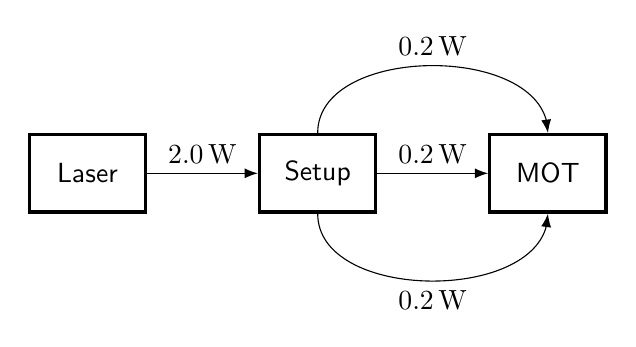
\begin{tikzpicture}[
				node distance=40pt,
				block/.style={draw, very thick, align=center, minimum height=28pt, minimum width=42pt}
			]
				\node[block] (laser) {Laser};
				\node[block, right=of laser] (setup) {Setup};
				\node[block, right=of setup] (mot) {MOT};
				\draw[-Latex] (laser) -- (setup) node[midway, above] {\SI{2.0}{\watt}};
				\draw[-Latex] (setup) -- (mot) node[midway, above] {\SI{0.2}{\watt}};

				\draw[-Latex] (setup.north) to[out=90, in=90] node[midway, above] {\SI{0.2}{\watt}} (mot.north);
				\draw[-Latex] (setup.south) to[out=-90, in=-90] node[midway, below] {\SI{0.2}{\watt}} (mot.south);
			\end{tikzpicture}
			\caption{Block diagram of the \SI{556}{\nano\meter} setup.}
		\end{figure}

	  \end{columns}
	\end{frame}
	
	% remarks:
	% - telescopes were only necessary because problems with the fibers
	% - photodiodes were not included
	\begin{frame}{Possible optical free-space setup}
		\begin{figure}
			\centering
			\includegraphics[scale=0.1]{556-implementation.pdf}
			\caption{Optical free-space setup of the \SI{556}{\nano\meter} setup by Clara (SQM lab).}
		\end{figure}
	\end{frame}
	
	\begin{frame}{Discussion}
		\begin{itemize}
			\item Use commercial shutters instead of selfmade shutters?
		\end{itemize}
	\end{frame}
	
	\appendix
	
	\begin{frame}{Double pass (cat-eye) AOM}
		
	\end{frame}
\end{document}